% !TeX root = paper.tex
\section{Experiment: Elementary Perceptual Tasks}

Cleveland and McGill describe a set of elementary graphical perceptual tasks across ten encodings, where each encodes a quantitative variable in a graphical element or visual mark~\cite{cleveland_mcgill,cleveland1985graphical}. These tasks are the low-level building blocks for information visualizations (Table~\ref{tab:encoding_parameters}): estimating position on a common scale, position on non-aligned scales, length, direction (or slope), angle, area, volume, curvature,  shading (or ink density), and color saturation. As human color perception is complex, and because Cleveland and McGill perform no experiments with it, for now we leave it for future work. 

For the remaining nine tasks, we create visualizations as 100$\times$100 raster images, and test whether each of our networks is able to regress absolute values from the images. As discussed in Section~\ref{sec:measuresandanalysis}, we generate multiple parameterizations for each elementary perceptual task to allow us to increase the number of parameters that the networks must estimate, and to measure performance as we move closer towards a general representation of visual marks. For instance, for \emph{Position Common Scale}, first we only vary the $y$-position of the spot to estimate against the scale, then we include translation along the x-axis, and then we vary the size of the spot size (Table~\ref{tab:encoding_parameters}). These parameterizations are still simple---each increase is only slightly more complex for a human to solve---but it increases the number of possible images for the network to `learn'.


%Cleveland and McGill did not explicitly test human perception of single instances of these encodings. -> JT: We now know this isn't true.

%\begin{figure}[t]
%	  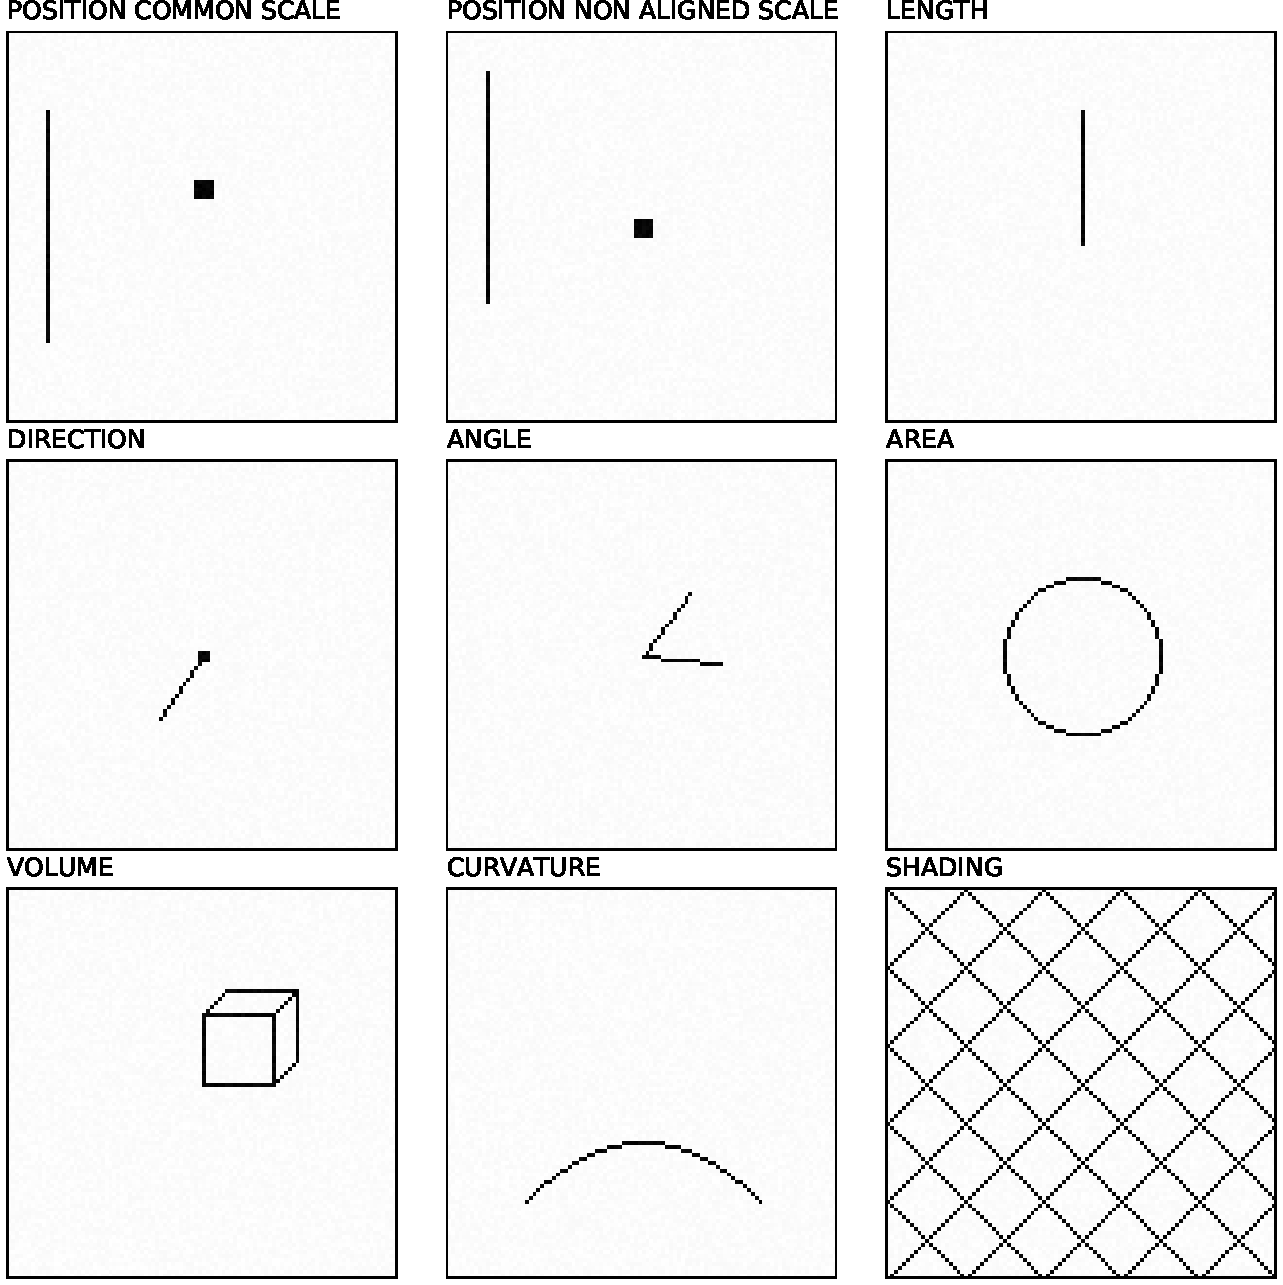
\includegraphics[width=\linewidth]{figure1_overview.pdf}
%  \caption{\textbf{Elementary Perceptual Tasks.} Rasterized visualizations of the elementary perceptual tasks as defined by Cleveland and McGill~\cite{cleveland_mcgill} (color saturation excluded). We vary the parameters of each perceptual task and then assess the interpretability of feed-forward neural networks.}
%	\label{fig:elementary_perceptual_tasks}
%\end{figure}



\begin{table}[!ht]
\centering
\caption{\textbf{Elementary Perceptual Tasks.} Rasterized visualizations of the elementary perceptual tasks as defined by Cleveland and McGill~\cite{cleveland_mcgill} (color saturation excluded). We sequentially increase the number of parameters for every task (e.g., by adding translation). This introduces variability and creates increasingly more complex datasets.}
\resizebox{\linewidth}{!}{
\begin{tabular}{lllr}
	\toprule
	\multicolumn{2}{l}{Elementary Perceptual Task} & ~ & Permutations\\
	\midrule
	\raisebox{-.85\height}{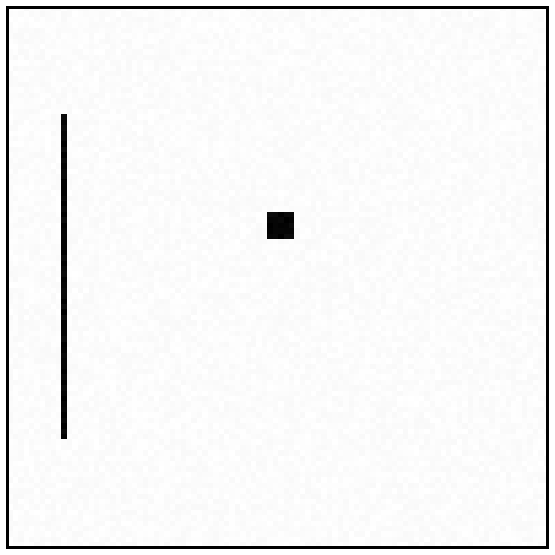
\includegraphics[width=.5in]{position_common_scale.pdf}} & \makecell[tl]{\emph{Position Common Scale}\\~~~Position Y\\~~~+ Position X \\~~~+ Spot Size \\} &~& \makecell[tr]{~\\ $60$ \\ $3,600$ \\ $216,00$}\\

	\midrule
	\raisebox{-.85\height}{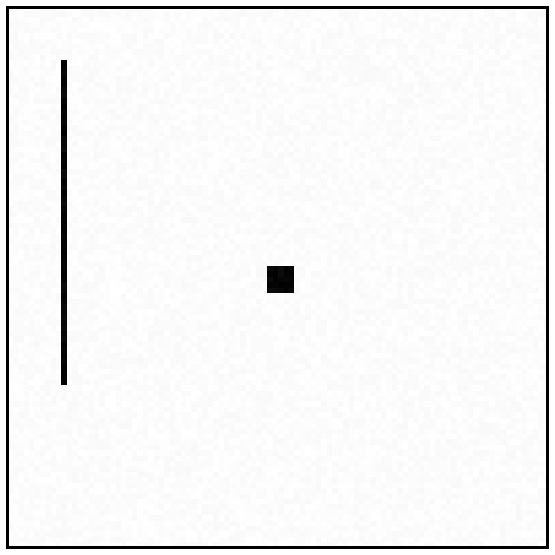
\includegraphics[width=.5in]{position_non_aligned_scale.pdf}} & \makecell[tl]{\emph{Position Non-Aligned Scale}\\~~~Position Y\\~~~+ Position X \\~~~+ Spot Size \\} &~& \makecell[tr]{~\\ $600$ \\ $36,000$ \\ $216,000$}\\

	\midrule
	\raisebox{-.95\height}{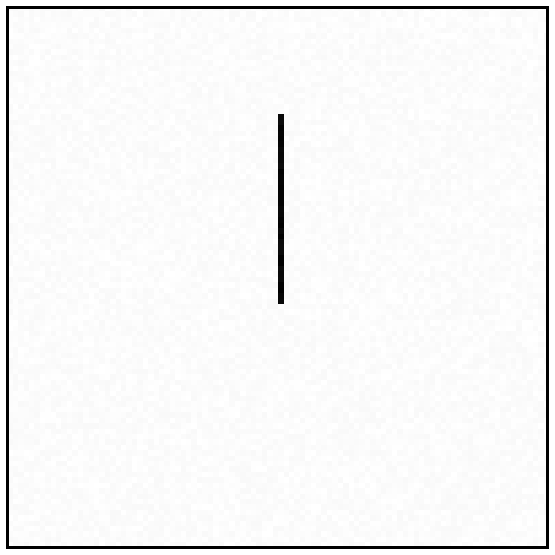
\includegraphics[width=.5in]{length.pdf}} & \makecell[tl]{\emph{Length}\\~~~Length\\~~~+ Position Y \\~~~+ Position X \\~~~+ Width} &~& \makecell[tr]{ ~\\$60$ \\ $2,400$ \\ $144,000$\\$864,000$}\\

	\midrule
	\raisebox{-.85\height}{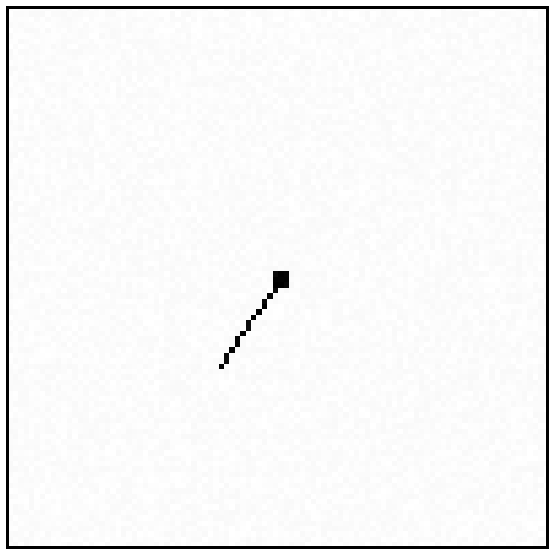
\includegraphics[width=.5in]{direction.pdf}} & \makecell[tl]{\emph{Direction}\\~~~Angle\\~~~+ Position Y \\~~~+ Position X} &~& \makecell[tr]{ ~\\$360$ \\ $21,600$ \\ $1,296,000$}\\

	\midrule
	\raisebox{-.85\height}{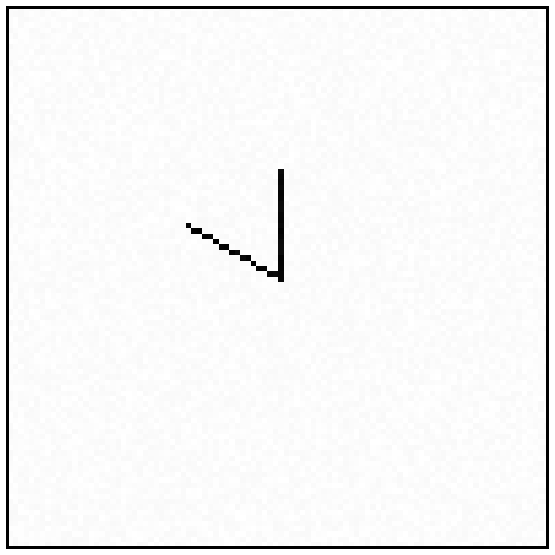
\includegraphics[width=.5in]{angle.pdf}} & \makecell[tl]{\emph{Angle}\\~~~Angle\\~~~+ Position Y \\~~~+ Position X} &~& \makecell[tr]{ ~\\$90$ \\ $5,400$ \\ $324,000$}\\

	\midrule
	\raisebox{-.85\height}{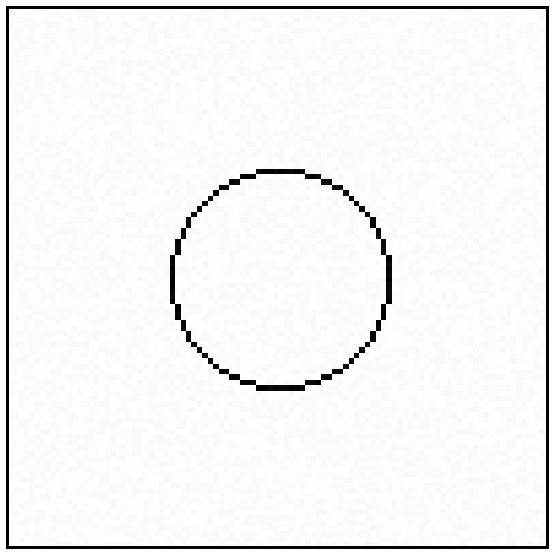
\includegraphics[width=.5in]{area.pdf}} & \makecell[tl]{\emph{Area}\\~~~Radius\\~~~+ Position Y \\~~~+ Position X} &~& \makecell[tr]{ ~\\$40$ \\ $800$ \\ $16,000$}\\

	\midrule
	\raisebox{-.85\height}{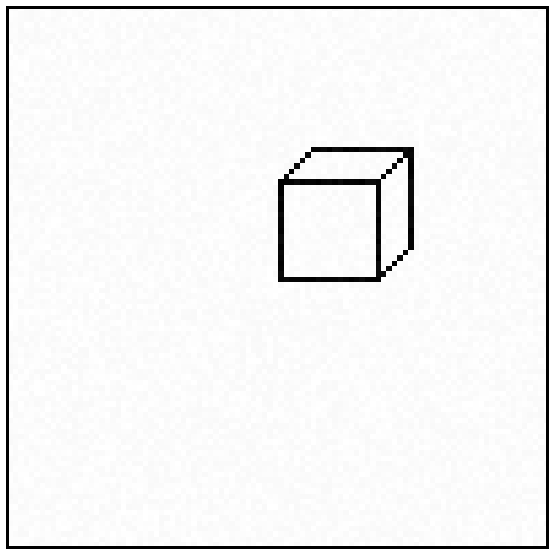
\includegraphics[width=.5in]{volume.pdf}} & \makecell[tl]{\emph{Volume}\\~~~Cube Sidelength\\~~~+ Position Y \\~~~+ Position X} &~& \makecell[tr]{ ~\\$20$ \\ $400$ \\ $8,000$}\\
	
	\midrule
	\raisebox{-.85\height}{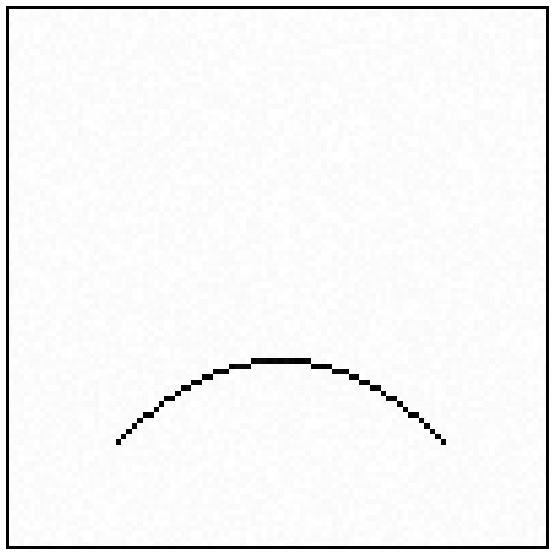
\includegraphics[width=.5in]{curvature.pdf}} & \makecell[tl]{\emph{Curvature}\\~~~Midpoint Curvature\\~~~+ Position Y \\~~~+ Position X} &~& \makecell[tr]{ ~\\$80$ \\ $1,600$ \\ $64,000$}\\	

	\midrule
	\raisebox{-.85\height}{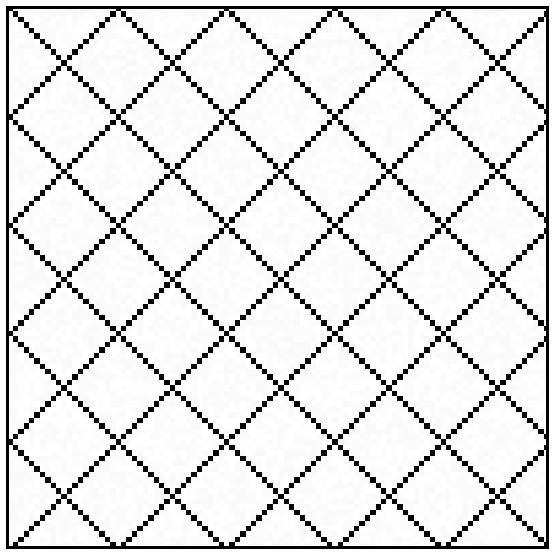
\includegraphics[width=.5in]{shading.pdf}} & \makecell[tl]{\emph{Shading}\\~~~Density\\~~~+ Position Y \\~~~+ Position X} &~& \makecell[tr]{ ~\\$100$ \\ $2,000$ \\ $40,000$}\\	
%	
	\bottomrule
\end{tabular}
}
\label{tab:encoding_parameters}
\end{table}



%
\subsection{Hypotheses}

\noindent \textbf{H1.1} \textbf{The CNNs tested will be able to regress quantitative variables from graphical elements.} We parametrize different visual encodings (Table~\ref{tab:encoding_parameters}) and test whether the CNNs can measure them, and relate the results to accuracies obtained by humans on similar tasks.

\noindent \textbf{H1.2} \textbf{CNN perceptual performance will depend on network architexture.} We evaluate multiple regressors with different numbers of trainable parameters. We expect a more complex network (with more trainable parameters) to perform better on elementary perceptual tasks.

\noindent \textbf{H1.3} \textbf{Some visual encodings will be easier to learn than others for the CNNs tested.} Cleveland and McGill order the elementary perceptual tasks by accuracy. We investigate whether this order is also relevant for computing graphical perception.

\noindent \textbf{H1.4} \textbf{Networks trained on perceptual tasks will generalize to more complex variations of the same task.} Empirical evidence suggests that CNNs are able to generalize by interpolating between different training data points, and so perform on variations of a similar perceptual task. We create visual representations of the elementary perceptual tasks with different variability, and expect that networks will be able to generalize when presented with slight task variations.

%	
%	We suspect that CNNs are able to 'learn` absolute quantities encoded using low-level visual 
%	
%	While much simpler models than their biological pendant, convolutional neural networks are heavily influenced by our biological knowledge of the visual system. Such classifiers therefor follow the same principles as human perception.


\subsection{Results}

% These values are similar or better than the range of MLAE=$3.02$--$3.82$ ($8-14\%$ error) for a similar experiment by Cleveland and McGill testing human estimation of relations between elementary perceptual tasks~\cite{cleveland1985graphical}. 

%While the performance varies for the different encodings, we observe for all networks performance similar to the measured human performance by Cleveland and McGill~\cite{cleveland1985graphical}. These results confirm our initial hypotheses.
\noindent{\textbf{Overall Accuracy.}} The tested CNNs and MLP are able to regress the visually encoded quantities in most cases (Fig.~\ref{fig:figure1_results}), with average error across all classifiers and tasks as \textit{MLAE}$=1.597$ ($SD=0.394$). % and \textit{MAE}=$2.89$ ($SD=0.848$). 
From these results, we \textbf{accept H1.1}.
\\~\\
\noindent{\textbf{Comparing Networks.}} 
Across network architectures and training schemes, there is considerable difference in performance. In order of decreasing error: 
The MLP has \textit{MLAE}$=2.943$ ($SD=0.857$), 
for LeNet $2.125$ ($SD=0.38$), 
Xception trained on ImageNet $1.627$ ($SD=0.462$), 
Xception trained from scratch $1.504$ ($SD=0.493$),
VGG19 trained on ImageNet $0.979$ ($SD=0.581$), 
and VGG19 trained from scratch $0.404$ ($SD=0.407$).

Across tasks, we compare the average regression performances for our networks and report the effect of the network as statistically significant ($F_{5,48}=20.392,p<0.01$). Post hoc comparisons show that the differences between LeNet and the VGG19 network, independent of the used weights, are significant ($t_48=4.674,p<0.01$). VGG19 from scratch and Xception (both versions) perform significantly differently, with Xception from scratch ($t_48=4.87,p<0.01$) and Xception with ImageNet weights ($t_48=5.621,p<0.01$). However, differences between LeNet and both Xception networks are not significant. Taken collectively, we \textbf{partially accept H1.2}, in that more tunable parameters does not automatically infer greater performance.
\\~\\
\noindent{\textbf{Ranking of Visual Encodings.}} Cleveland and McGill provide an ordering of elementary visual encodings based on theoretical arguments and experimental results. We compare their ranking with rankings of our networks in Table~\ref{tab:ranking}. Overall, there is significant variability in the rankings between architectures (Fig.~\ref{fig:figure1_results}). However, area estimation is an easier task for all networks, while direction and angle estimation are more difficult. It is harder to distinguish differences between position, length, curvature, and shading tasks. Further, the volume tasks suffers high variability in performance across cross-validation splits, which suggests that the image noise affects the outcome more than for other tasks. In sum, we \textbf{partially accept H1.3}. Finally, we note that the rankings between networks using ImageNet weights is identical, which suggests that the information about elementary perceptual tasks gained from those natural images is similar (given a sufficiently-complex network).
\\~\\
\noindent{\textbf{Cross-network Variability and Network Generalizability.}} We measure regression performance across networks trained with different parameterizations of the elementary perceptual tasks (Fig.~\ref{fig:cross_network}). For our best performing network (VGG19 trained from scratch), we observe that accuracy decreases only slightly as the parameterization becomes more complex so long as training examples expressing all variability are included (diagonal entries in each matrix).  However, VGG19 is unable to generalize to added translation or stroke width variations in the encodings, leading to increases in error. As such, we \textbf{reject H1.4}. 

%Observing Figure~\ref{fig:figure1_results}, -> JT: we should do this.

%Since such a ranking see,s to heavily depend on the used regressor, the weights, and the initialization, we do not think a generalized ranking can be created and \textbf{reject H1.3}.

\begin{table}[tb]
\centering
\caption{\textbf{Elementary Perceptual Task Ranking.} We report midmean logistic absolute errors (MLAE) for each network averaged across multiple runs on the most complex parametrization of each task. For human performance, we report the ranking of Cleveland and McGill~\cite{cleveland_mcgill}. VGG19 performs best overall, while VGG19 * and Xception * networks using ImageNet weights yield identical rankings.}
\resizebox{\linewidth}{!}{
\begin{tabular}{cllllll}
\toprule
Human (CMcG) & MLP & LeNet & VGG19 * & \textbf{VGG19} & Xception * & Xception \\
\midrule
\multicolumn{7}{l}{\emph{Position Common Scale}} \\
1. & 7. (3.84) & 2. (1.36) & 5. (1.02) & \textbf{3.} (-0.04) & 5. (1.65) & 1. (1.04)\\
\multicolumn{7}{l}{\emph{Position Non aligned Scale}} \\
2. & 6. (3.61) & 1. (1.35) & 6. (1.09) & \textbf{5.} (0.26) & 6. (1.71) & 2. (1.06)\\
\multicolumn{7}{l}{\emph{Length}} \\
3. & 1. (1.99) & 8. (3.19) & 4. (0.87) & \textbf{2.} (-0.14) & 4. (1.59) & 3. (1.11) \\
\multicolumn{7}{l}{\emph{Direction}} \\
3. & 9. (4.65) & 7. (3.07) & 9. (2.84) & \textbf{8.} (0.92) & 9. (3.46) & 6. (1.57) \\
\multicolumn{7}{l}{\emph{Angle}} \\
3. & 8. (4.61) & 9. (3.33) & 8. (2.31) & \textbf{9.} (0.99) & 8. (2.60) & 7. (1.72) \\
\multicolumn{7}{l}{\emph{Area}} \\
4. & 2. (2.01) & 5. (2.21) & 1. (0.49) & \textbf{1.} (-0.17) & 1. (0.80) & 5. (1.38) \\
\multicolumn{7}{l}{\emph{Volume}} \\
5. & 4. (2.38) & 4. (1.91) & 7. (1.16) & \textbf{7.} (0.87) & 7. (2.03) & 9. (2.10) \\
\multicolumn{7}{l}{\emph{Curvature}} \\
5. & 3. (2.34) & 3. (1.81) & 2. (0.71) & \textbf{6.} (0.28) & 2. (1.17) & 4. (1.13) \\
\multicolumn{7}{l}{\emph{Shading}} \\
6. & 5. (3.04) & 6. (2.23) & 3. (0.73) & \textbf{4.} (0.14) & 3. (1.57) & 8. (1.82) \\

% 
%\makecell[tl]{\emph{Position}\\~~\emph{Non-aligned Scale}} & 1 & 1 & 2 & 3 & \textbf{4} & 5 & 6 \\
%\makecell[tl]{\emph{Length}} & 1 & 1 & 2 & 3 & \textbf{4} & 5 & 6 \\
%\makecell[tl]{\emph{Direction}} & 1 & 1 & 2 & 3 & \textbf{4} & 5 & 6 \\
%\makecell[tl]{\emph{Angle}} & 1 & 1 & 2 & 3 & \textbf{4} & 5 & 6 \\
%\makecell[tl]{\emph{Area}} & 1 & 1 & 2 & 3 & \textbf{4} & 5 & 6 \\
%\makecell[tl]{\emph{Volume}} & 1 & 1 & 2 & 3 & \textbf{4} & 5 & 6 \\
%\makecell[tl]{\emph{Curvature}} & 1 & 1 & 2 & 3 & \textbf{4} & 5 & 6 \\
%\makecell[tl]{\emph{Shading}} & 1 & 1 & 2 & 3 & \textbf{4} & 5 & 6 \\
%\begin{tabular}{ll}
%	\toprule
%	Task & \begin{tabular}{ccccccc}
%			Human & MLP & LeNet & VGG19 * & VGG19 & Xception * & Xception
%			\end{tabular}\\
%	\midrule
%	\raisebox{-.85\height}{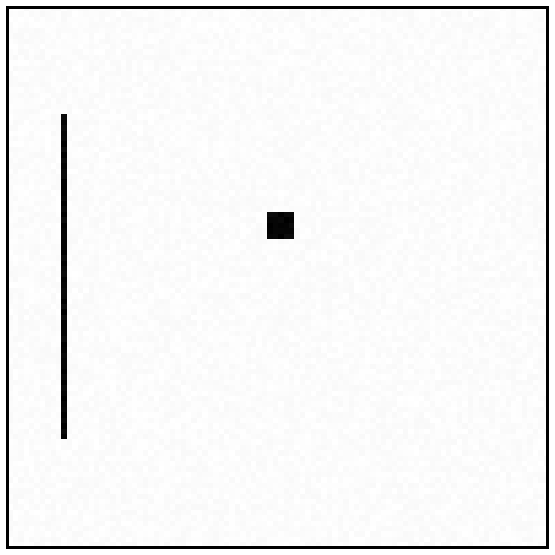
\includegraphics[width=.5in]{position_common_scale.pdf}} & \makecell[tl]{\emph{Position Common Scale}\\ \begin{tabular}{ccccccc}
%
%\end{tabular}} \\
%
%	\midrule
%	\raisebox{-.85\height}{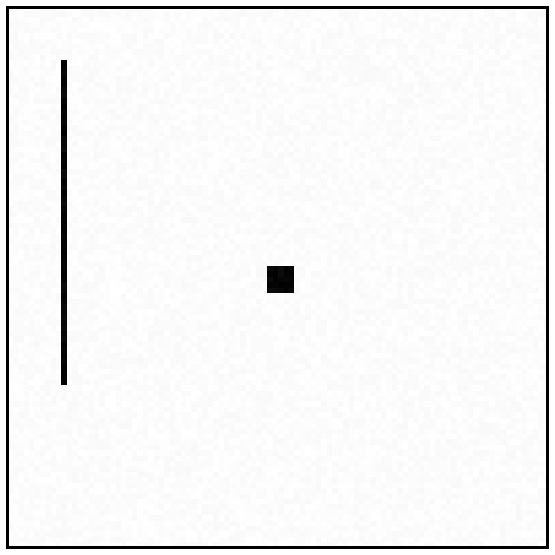
\includegraphics[width=.5in]{position_non_aligned_scale.pdf}} & \makecell[tl]{\emph{Position Non-Aligned Scale}\\~~~Position Y\\~~~+ Position X \\~~~+ Spot Size \\} &~& \makecell[tr]{~\\ $600$ \\ $36,000$ \\ $216,000$}\\
%
%	\midrule
%	\raisebox{-.95\height}{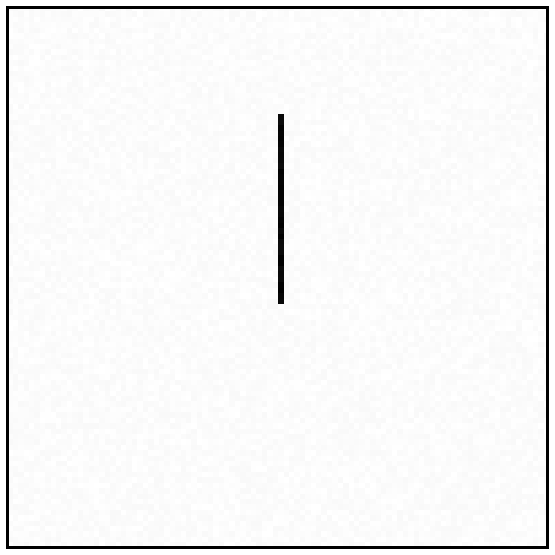
\includegraphics[width=.5in]{length.pdf}} & \makecell[tl]{\emph{Length}\\~~~Length\\~~~+ Position Y \\~~~+ Position X \\~~~+ Width} &~& \makecell[tr]{ ~\\$60$ \\ $2,400$ \\ $144,000$\\$864,000$}\\
%
%	\midrule
%	\raisebox{-.85\height}{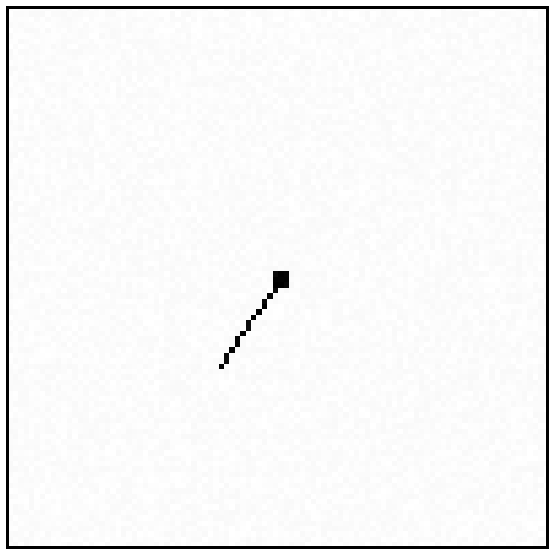
\includegraphics[width=.5in]{direction.pdf}} & \makecell[tl]{\emph{Direction}\\~~~Angle\\~~~+ Position Y \\~~~+ Position X} &~& \makecell[tr]{ ~\\$360$ \\ $21,600$ \\ $1,296,000$}\\
%
%	\midrule
%	\raisebox{-.85\height}{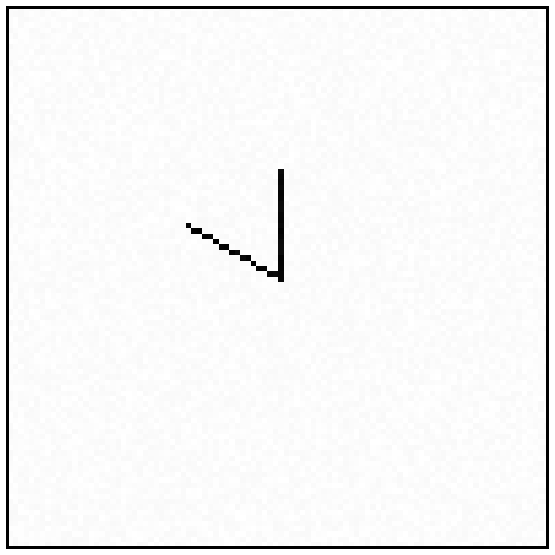
\includegraphics[width=.5in]{angle.pdf}} & \makecell[tl]{\emph{Angle}\\~~~Angle\\~~~+ Position Y \\~~~+ Position X} &~& \makecell[tr]{ ~\\$90$ \\ $5,400$ \\ $324,000$}\\
%
%	\midrule
%	\raisebox{-.85\height}{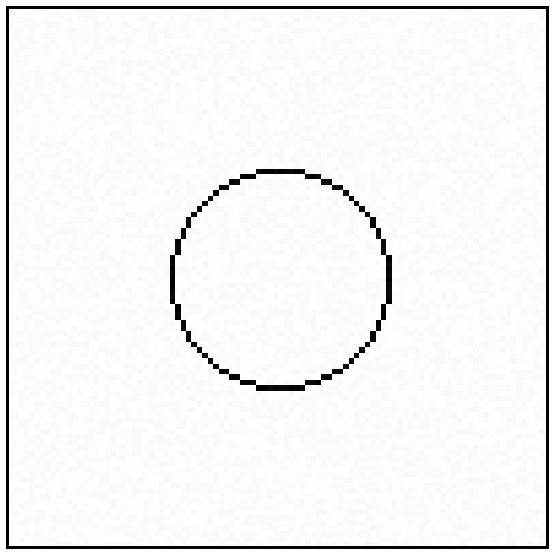
\includegraphics[width=.5in]{area.pdf}} & \makecell[tl]{\emph{Area}\\~~~Radius\\~~~+ Position Y \\~~~+ Position X} &~& \makecell[tr]{ ~\\$40$ \\ $800$ \\ $16,000$}\\
%
%	\midrule
%	\raisebox{-.85\height}{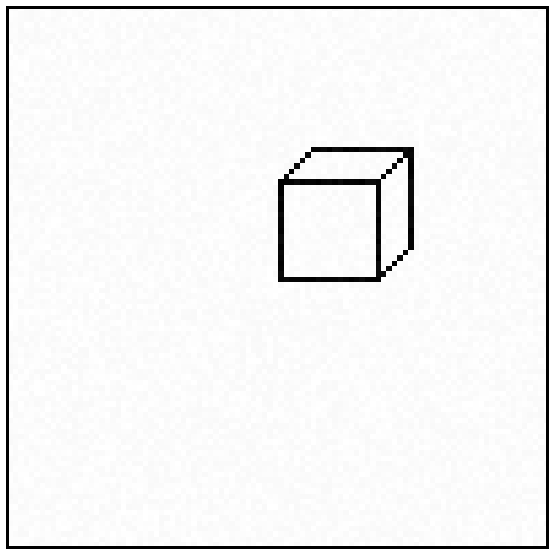
\includegraphics[width=.5in]{volume.pdf}} & \makecell[tl]{\emph{Volume}\\~~~Cube Sidelength\\~~~+ Position Y \\~~~+ Position X} &~& \makecell[tr]{ ~\\$20$ \\ $400$ \\ $8,000$}\\
%	
%	\midrule
%	\raisebox{-.85\height}{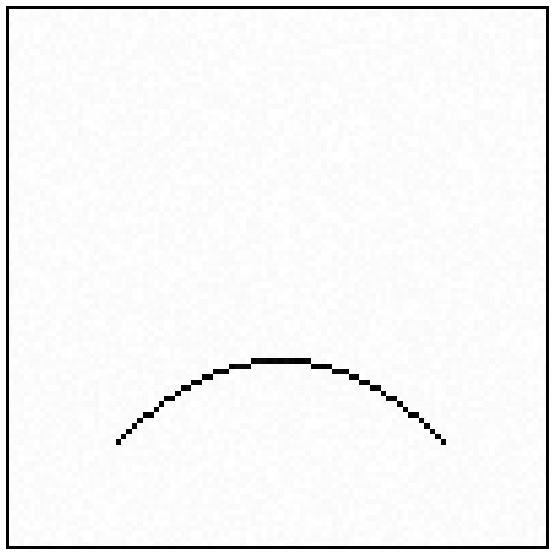
\includegraphics[width=.5in]{curvature.pdf}} & \makecell[tl]{\emph{Curvature}\\~~~Midpoint Curvature\\~~~+ Position Y \\~~~+ Position X} &~& \makecell[tr]{ ~\\$80$ \\ $1,600$ \\ $64,000$}\\	
%
%	\midrule
%	\raisebox{-.85\height}{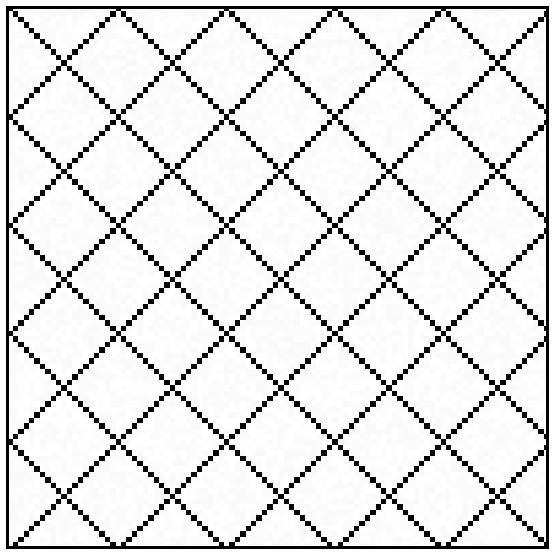
\includegraphics[width=.5in]{shading.pdf}} & \makecell[tl]{\emph{Shading}\\~~~Density\\~~~+ Position Y \\~~~+ Position X} &~& \makecell[tr]{ ~\\$100$ \\ $2,000$ \\ $40,000$}\\	

	\bottomrule
\end{tabular}
}
\label{tab:ranking}
\end{table}

\begin{figure}[p]
	\centering
	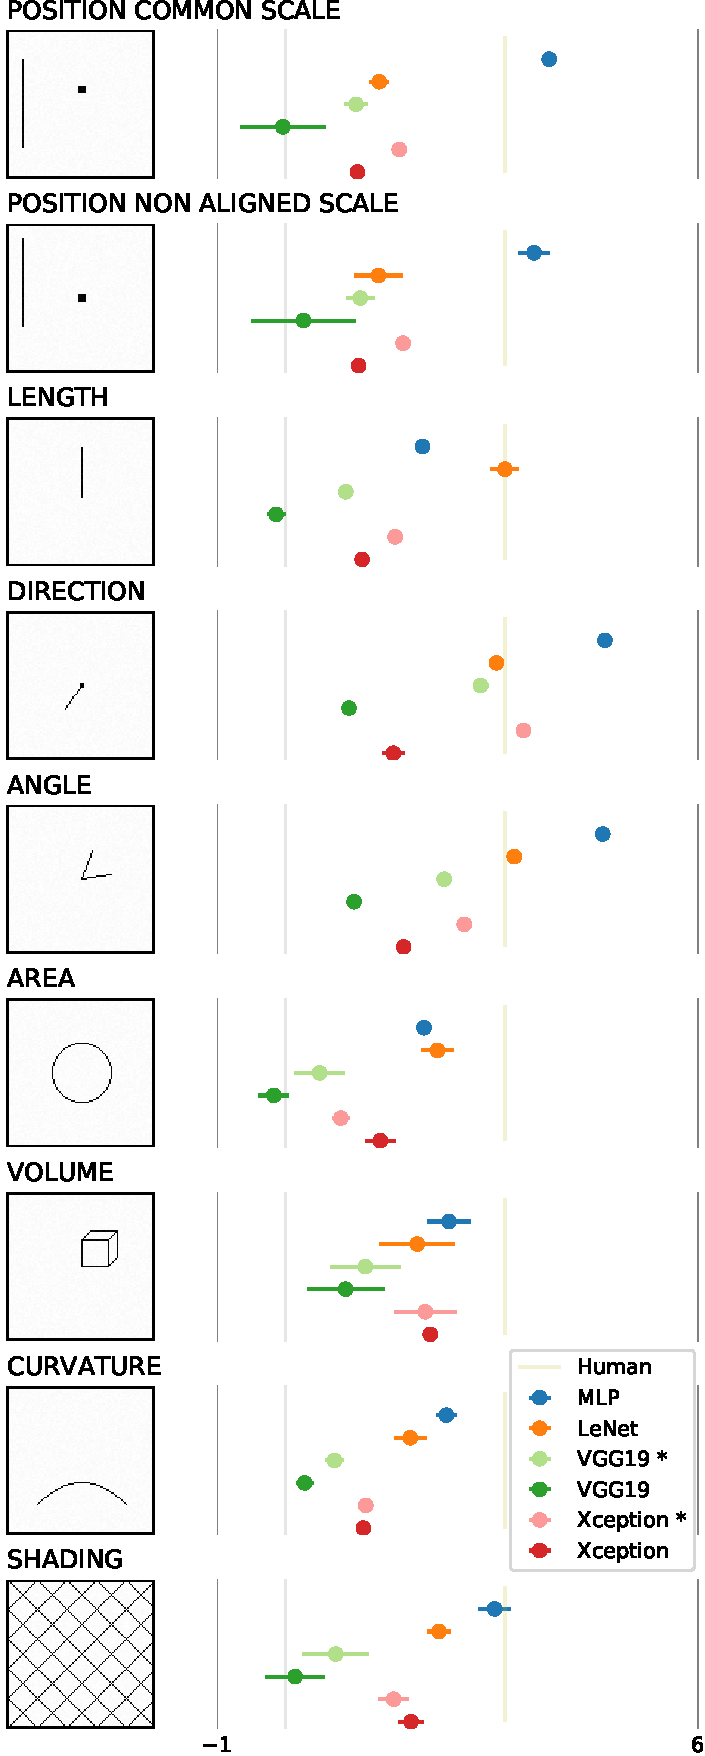
\includegraphics[width=\linewidth]{figure1_slim_only_last.pdf}
%	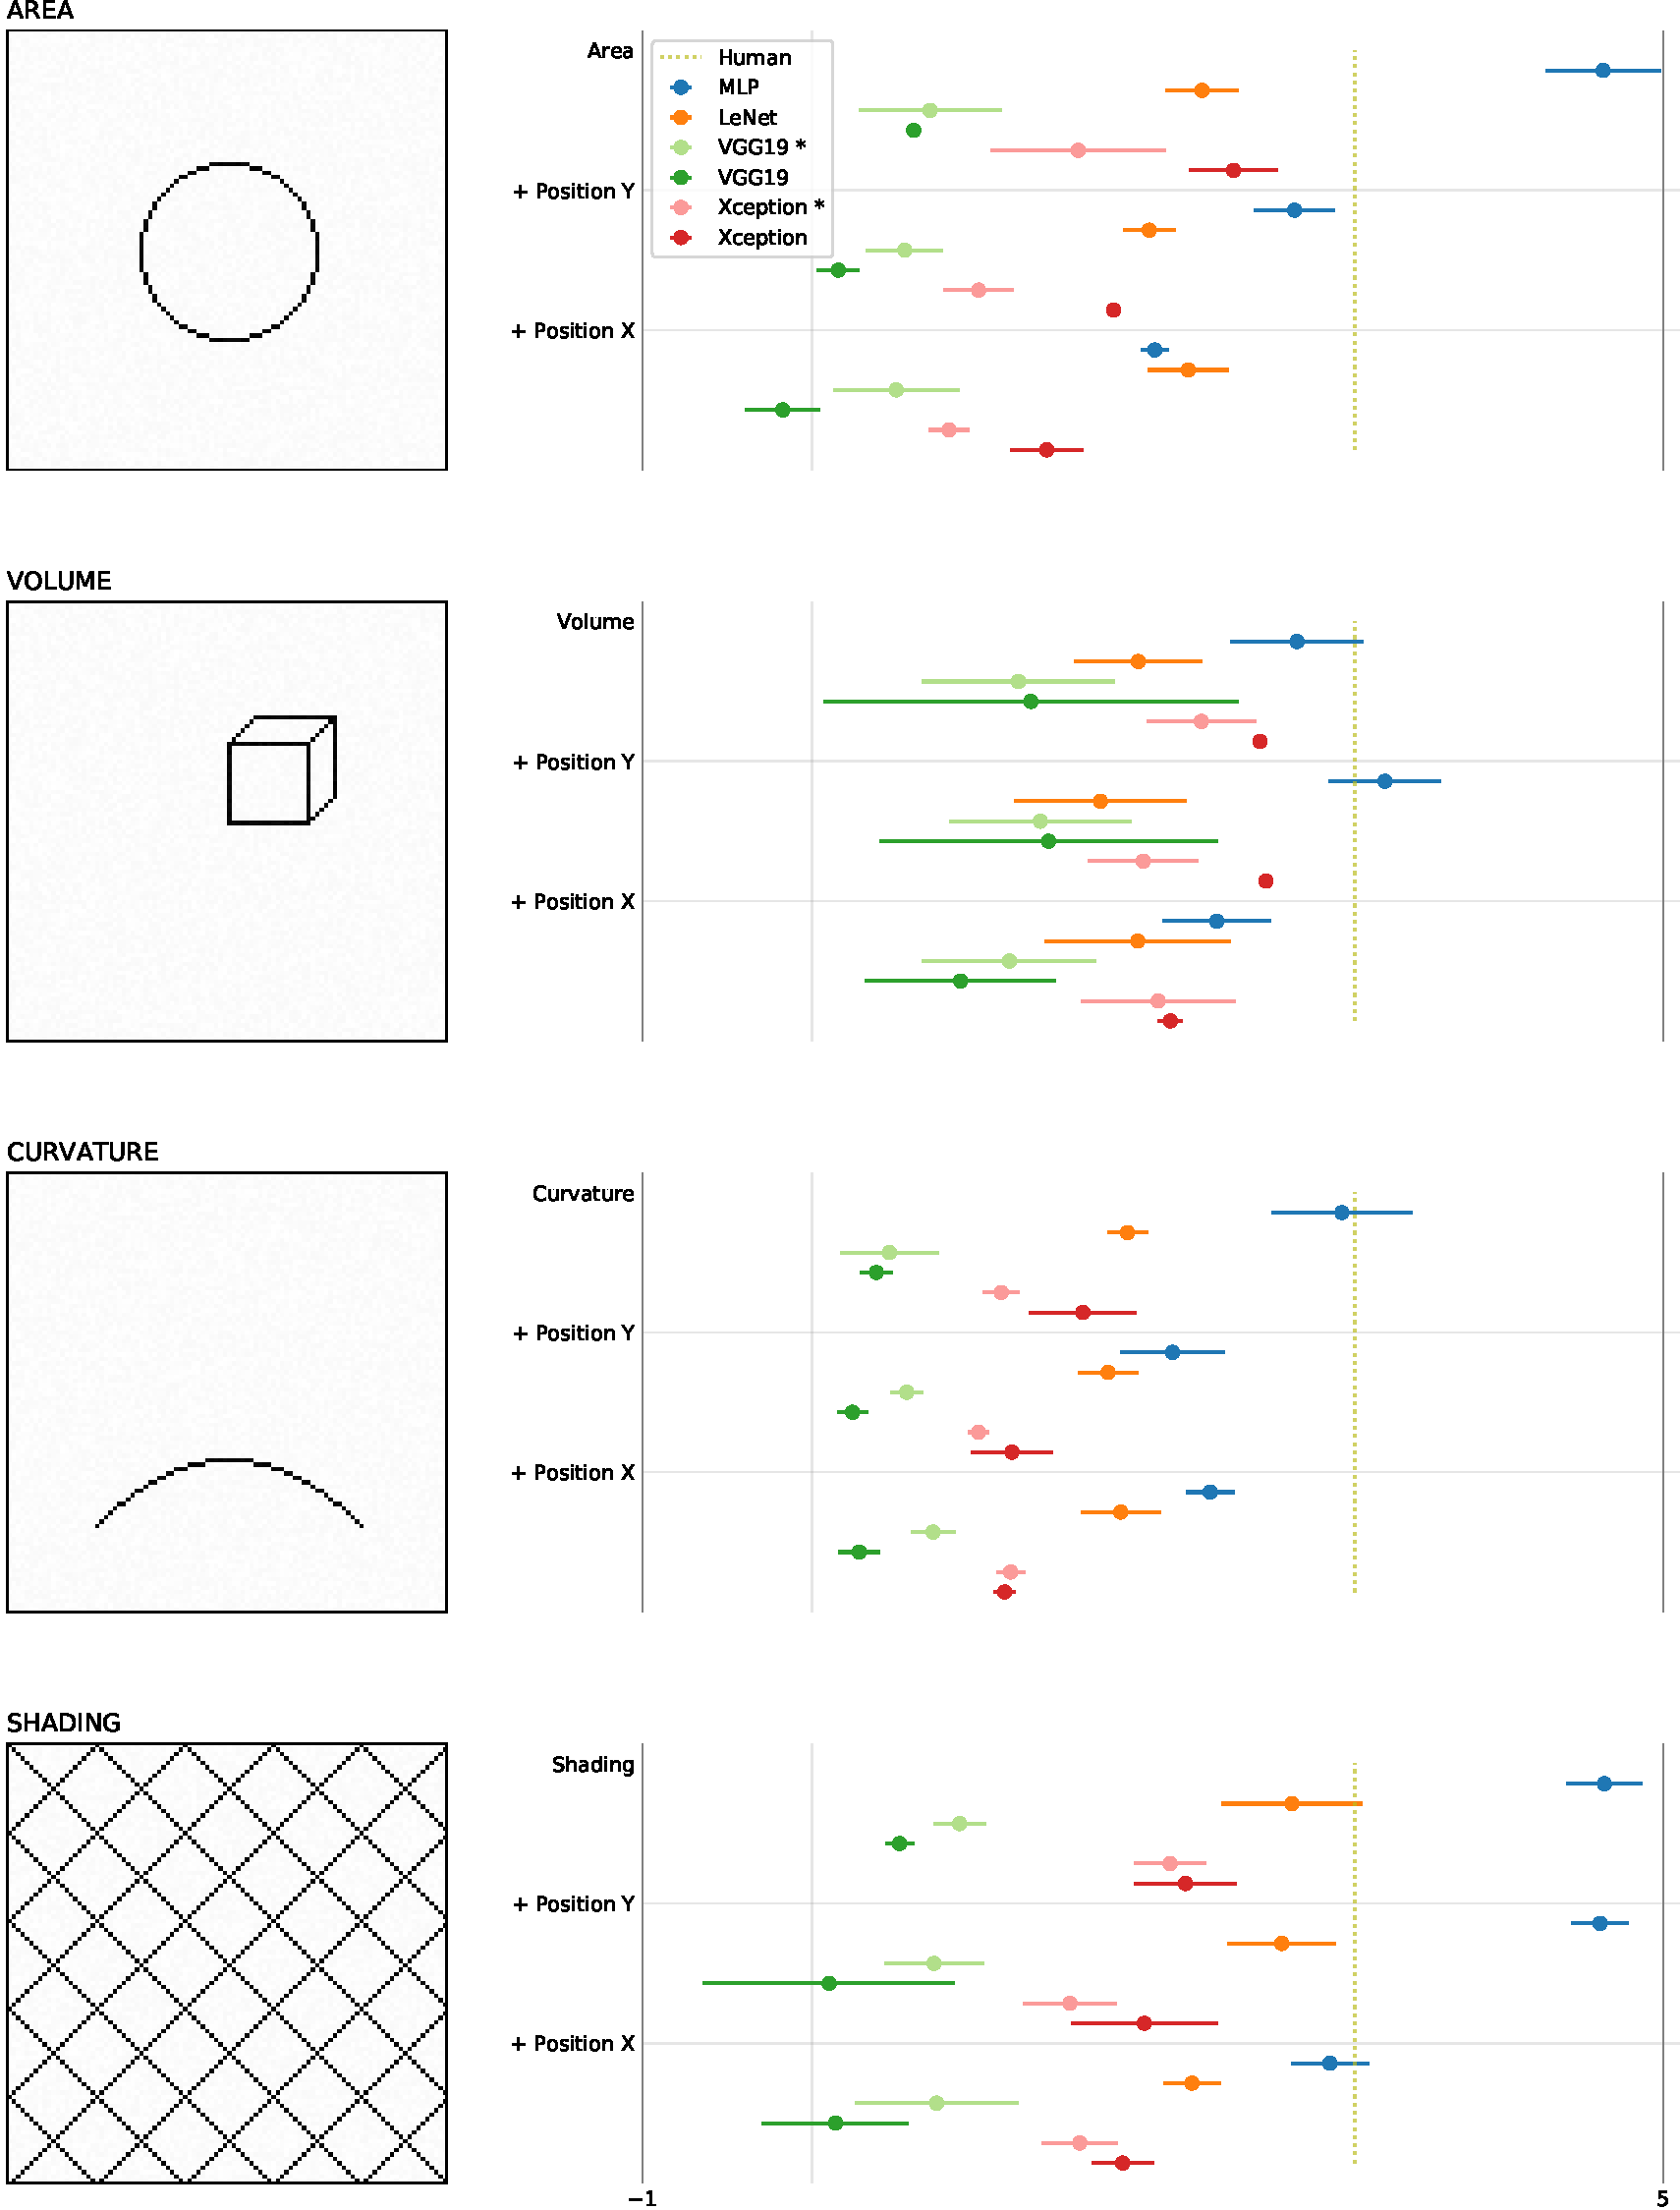
\includegraphics[width=0.48\linewidth]{figure1_slim_right.pdf}
	\caption{\textbf{Elementary perceptual tasks results for most complex task parameterization.} \emph{Left:} Example stimuli image. \emph{Right:} MLAE and 95\% confidence intervals for different networks. The * indicates networks which use ImageNet weights up until the MLP, rather than being trained from scratch.}
	\label{fig:figure1_results}
%	\vspace*{1in}
\end{figure}


\begin{figure}[p]
	\centering
	  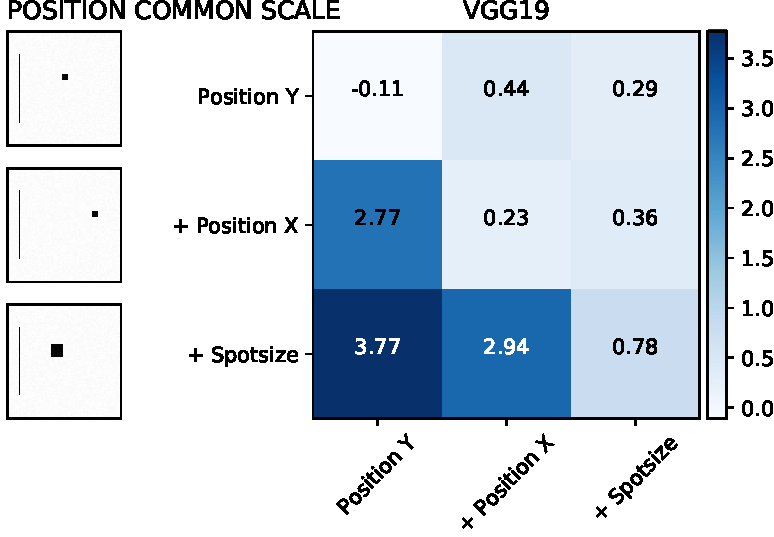
\includegraphics[width=.8\linewidth]{cross_network_small_VGG19_position_common_scale.pdf}
	  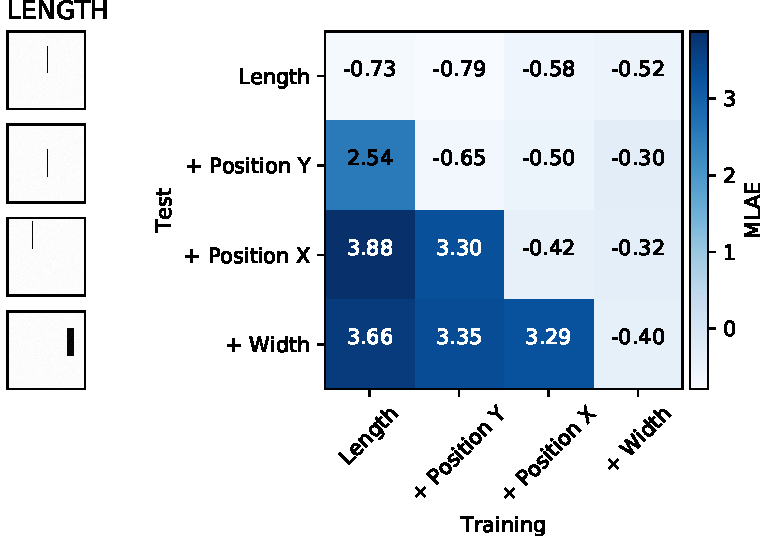
\includegraphics[width=.8\linewidth]{cross_network_small_VGG19_length.pdf}
	  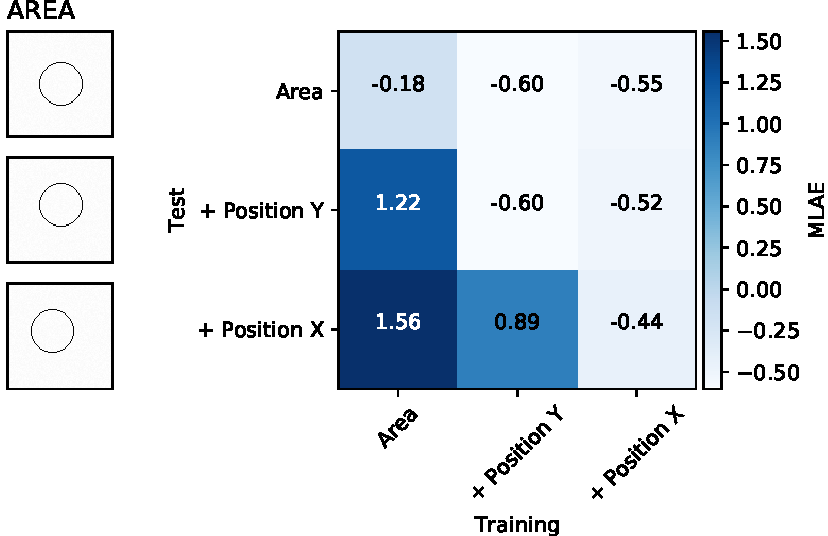
\includegraphics[width=.8\linewidth]{cross_network_small_VGG19_area.pdf}
	  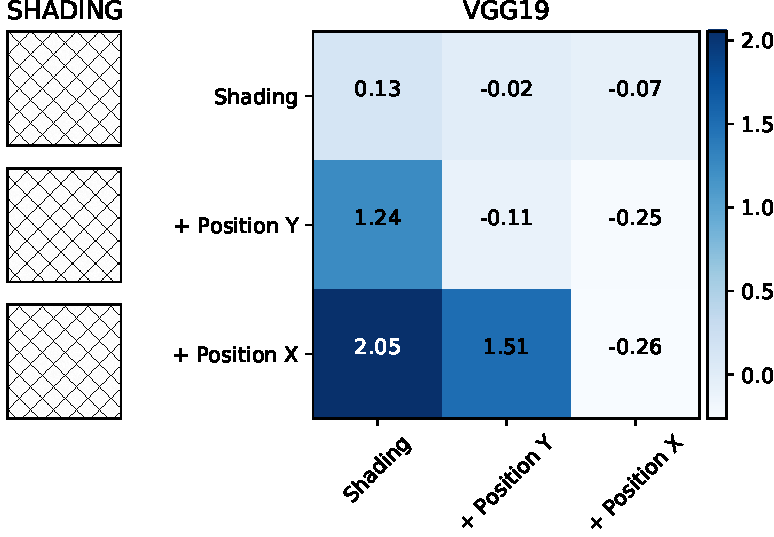
\includegraphics[width=.8\linewidth]{cross_network_small_VGG19_shading.pdf}
  \caption{\textbf{Cross-classifier variability for perceptual tasks.} VGG19 networks trained on different parametrizations (X-axis) tested across different parameterizations (Y-axis), for the top four performing encodings. Diagonal matrix entries represent networks trained and tested on the same parameterizations. Below diagonal entries are scenarios where the test data has more parameters than the training data; below diagonal entries have fewer. We measure the mean logistic absolute error (MLAE)---the lower the score, the better. VGG19 becomes only slightly less accurate as the parameterization becomes more complex; however, it is unable to generalize to unseen element translations as error increases rapidly. Note that all networks showed similar behavior.}
	\label{fig:cross_network}
\end{figure}

